\documentclass[11pt,a4paper]{article}

\usepackage[margin=2.2cm]{geometry}
\usepackage{amsmath,amssymb}
\usepackage{graphicx}
\usepackage{booktabs}
\usepackage{caption}
\usepackage{subcaption}
\usepackage{xcolor}
\usepackage{hyperref}
\usepackage{titlesec}

\hypersetup{colorlinks=true,linkcolor=blue!50!black,urlcolor=blue!50!black}
\titleformat{\section}{\large\bfseries\color{blue!40!black}}{\thesection}{0.6em}{}
\titleformat{\subsection}{\normalsize\bfseries}{\thesubsection}{0.6em}{}

\title{\bfseries Any-Order Autoregressive Transformer + GMM\\[2pt]
       \large An ICF-style probabilistic surrogate trained on \texttt{combined\_data.xlsx}}
\author{Generated with Claude Code}
\date{\today}

\begin{document}
\maketitle

\begin{abstract}
We re-implement the unified probabilistic model described in the slide deck
\emph{机器学习横版.pdf} and apply it to the dataset \texttt{combined\_data.xlsx}
(10\,000 samples, 5 inputs and 15 outputs). The model is a bidirectional
Transformer encoder with a Gaussian-mixture output head, trained with a
random masking ratio so that one network simultaneously approximates every
conditional density $p(\mathbf{x}_{S}\mid\mathbf{x}_{S^{c}})$ of the joint
distribution. A single trained checkpoint then serves as a forward surrogate
($\overline{R^{2}}\!=\!0.944$), an inverse surrogate, and a Bayesian
posterior generator. This reproduces the observations of the slide deck on
real data.
\end{abstract}

%==============================================================
\section{Background and motivation}

The slide deck (Pages 1--4) frames three classes of ICF design questions
\textemdash{} forward surrogate $p(\mathbf{y}\mid\mathbf{x})$, inverse design
$p(\mathbf{x}\mid\mathbf{y})$, and scaling-law analysis $p(\mathbf{y}_{2}\mid\mathbf{y}_{1})$
\textemdash{} as different conditional slices of the same joint distribution
$p(\mathbf{x},\mathbf{y})$. The proposed remedy is a single network that fits
every conditional, exploiting the chain-rule identity
\begin{equation}
  p(x_{1},\ldots,x_{n}) \;=\; \prod_{i=1}^{n} p\bigl(x_{\sigma(i)}\mid x_{\sigma(1)},\ldots,x_{\sigma(i-1)}\bigr)
  \label{eq:chain}
\end{equation}
for an arbitrary permutation $\sigma$. The architectural recipe (Page~4 of the deck)
is a bidirectional Transformer that ingests every variable as a token of the form
$[\mathit{value},\;\mathit{mask},\;\mathit{onehot\_id}]$ and outputs a
Gaussian-mixture density on each token. Random sub-set masking during training
makes the loss equivalent to minimising the KL divergence between the model
density and the data density (Goodfellow~2016).

%==============================================================
\section{Dataset}

The supplied file \texttt{combined\_data.xlsx} contains a single sheet of
$10\,000$ rows and $20$ float columns: \texttt{input-1}\,$\dots$\,\texttt{input-5}
followed by \texttt{output-1}\,$\dots$\,\texttt{output-15}. The values are
already approximately normalised. We split $9\,000$ rows for training and
$1\,000$ rows for testing (random seed $0$); the held-out indices are saved
in \texttt{artifacts/test\_indices.npy}.

%==============================================================
\section{Model}

The implementation lives in \texttt{model.py}. The same architecture as the
deck is used, with the dimension scaled down to keep CPU training under
4\,minutes. Per-token features
$\bigl[\,v_i,\;m_i,\;\mathrm{onehot}(i)\,\bigr]\in\mathbb{R}^{2+N}$ are
embedded by a linear layer and refined by $L$ pre-norm Transformer
encoder layers with full bidirectional attention; a per-token linear head
emits the parameters of a $K$-component Gaussian mixture, see
Eq.~\ref{eq:gmm}.
\begin{equation}
  p(x) \;=\; \sum_{k=1}^{K}\frac{w_k}{\sqrt{2\pi}\,\sigma_k}
              \exp\!\left(-\frac{(x-\mu_k)^{2}}{2\sigma_k^{2}}\right),
  \qquad \sum_k w_k = 1.
  \label{eq:gmm}
\end{equation}

\begin{table}[h]\centering\small
\begin{tabular}{lccccccc}
\toprule
 & $N$ & $d_{\text{model}}$ & layers & heads & $d_{\text{ff}}$ & $K$ & params \\\midrule
This work        & 20 & 64  & 4 & 4 & 256  & 10 & 0.20\,M \\
PPT reference    & 28 & 128 & 8 & 4 & --   & 20 & 1.6\,M  \\
\bottomrule
\end{tabular}
\caption{Architectural settings. The reduced configuration was chosen because
the present dataset has only 20 dimensions and we train on CPU.}
\end{table}

\paragraph{Loss.}
For every batch, a masking ratio $r\sim\mathcal{U}(1/N,\,1{-}1/N)$ is sampled
and an independent Bernoulli mask $\mathbf{m}\in\{0,1\}^{N}$ is drawn with
$\Pr(m_i{=}1)=r$. Hidden positions get their value zeroed but keep their
identity onehot. The loss is the negative log-likelihood averaged over the
masked positions only,
\begin{equation}
  \mathcal{L}(\theta) \;=\; -\frac{1}{|\mathcal{S}|}
        \sum_{i\in\mathcal{S}} \log p_\theta\bigl(x_i\,\big|\,\mathbf{x}_{\mathcal{S}^{c}}\bigr),
\end{equation}
which, when averaged over $r\sim\mathcal{U}(0,1)$ and the data, is an
unbiased estimator of the negative log-likelihood of the joint density.

\paragraph{Optimisation.}
AdamW ($\eta=2{\times}10^{-3}$, weight-decay $10^{-5}$), cosine LR schedule,
gradient norm clipped to $1.0$, batch $256$, $120$ epochs, run on CPU.

%==============================================================
\section{Training dynamics}

Figure~\ref{fig:curves} shows the training and held-out NLL together with
the surrogate-mode RMSE. Forward and inverse RMSE drop in lock-step with the
likelihood, mirroring the right-hand panel of Page~7 of the deck.

\begin{figure}[h]\centering
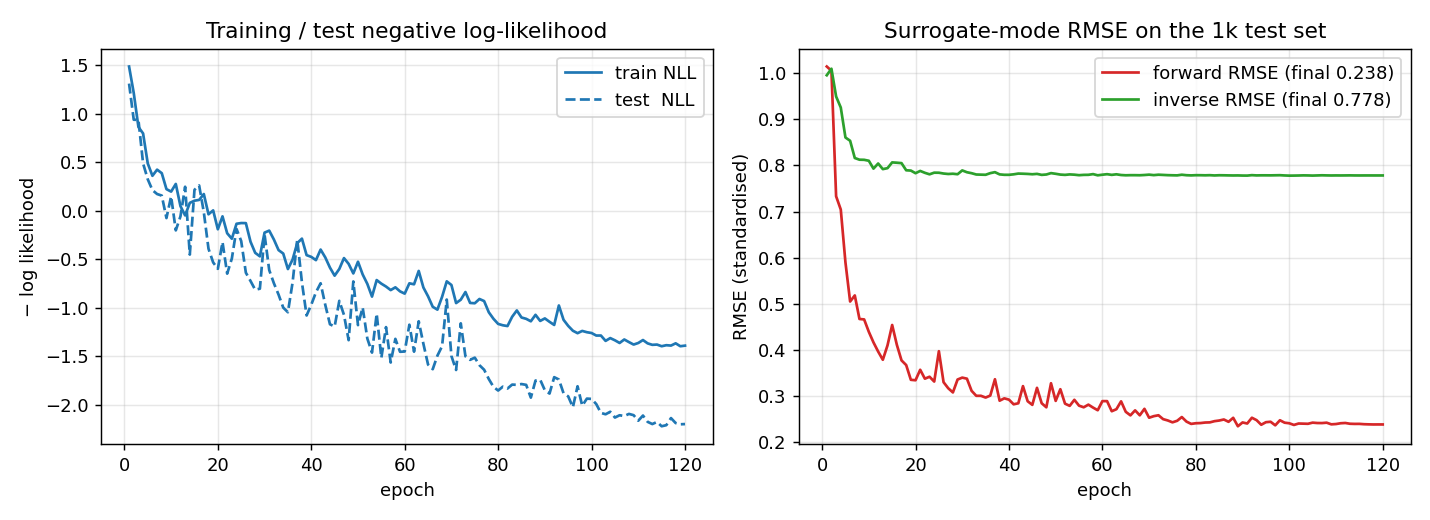
\includegraphics[width=0.95\linewidth]{artifacts/figs/01_training_curves.png}
\caption{Left: negative log-likelihood per epoch (solid = training, dashed =
test). Right: surrogate RMSE on the test set; the forward surrogate
converges quickly while the inverse surrogate plateaus higher, signalling
that the inverse problem is intrinsically multi-valued.}
\label{fig:curves}
\end{figure}

%==============================================================
\section{Marginal-density fit}

To check that the network has learned the joint, we compare the unconditioned
marginal $p(x_i)$ \textemdash{} obtained by feeding an all-mask token vector
\textemdash{} with the empirical histogram of every column. Figure~\ref{fig:marg}
shows that the GMM heads recover the correct shape (uni-, bi-modal, skewed
tails) for all 20 quantities, just as on Page~6 of the slide deck.

\begin{figure}[h]\centering
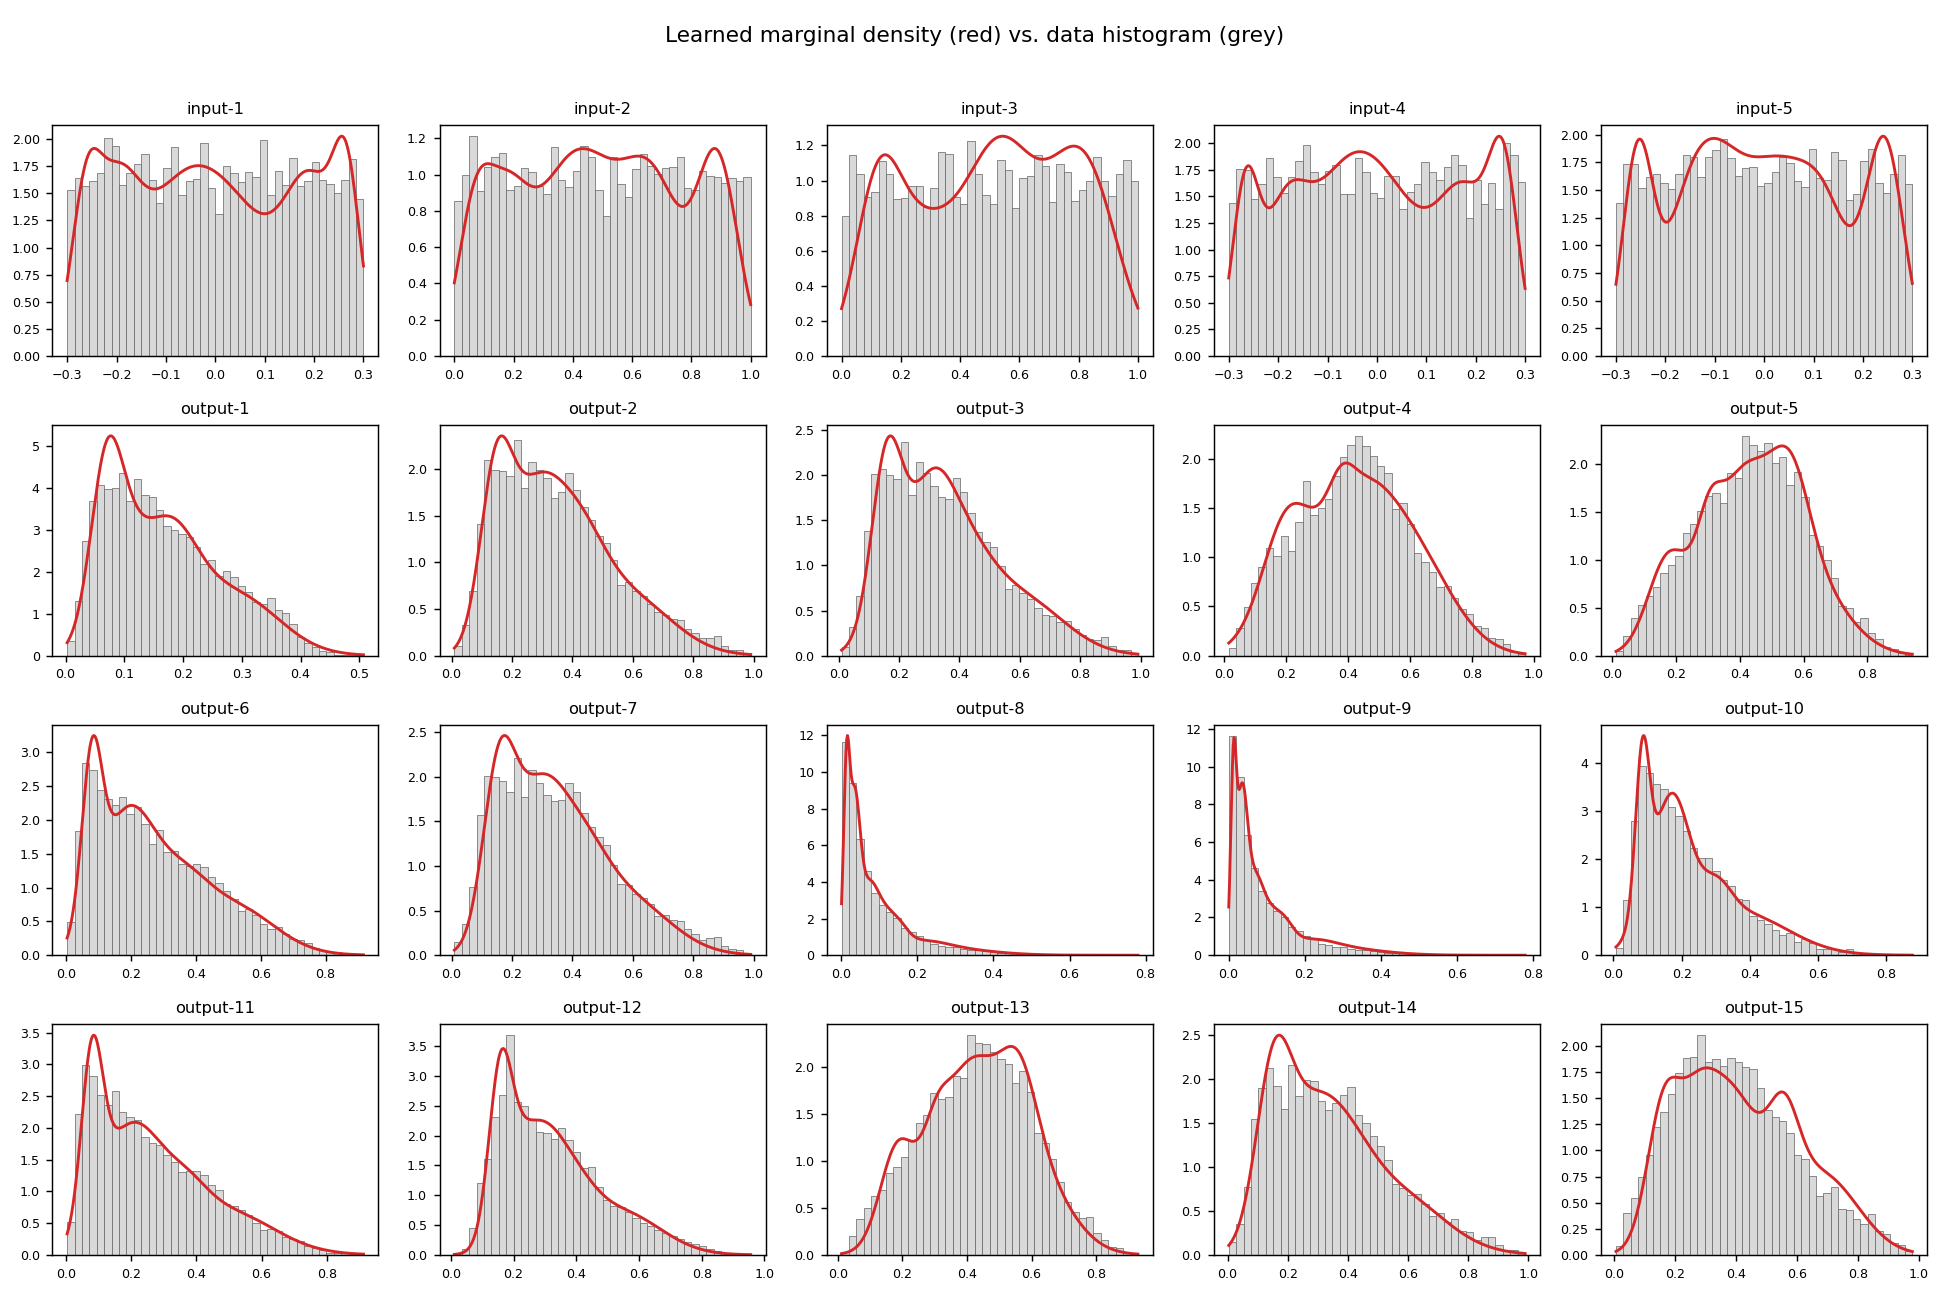
\includegraphics[width=0.97\linewidth]{artifacts/figs/02_marginals.png}
\caption{Learned marginal density (red) vs.\ data histograms (grey) for each
of the 20 quantities. The red curves are obtained from a single forward
pass with all tokens masked.}
\label{fig:marg}
\end{figure}

%==============================================================
\section{Forward surrogate mode}

Setting the 5 inputs as visible and the 15 outputs as masked, the per-token
GMM means $\sum_k w_k \mu_k$ are taken as point estimates of the outputs.
Across the held-out test set the average performance is
\[
  \overline{R^{2}}_{\text{fwd}} = 0.944,\qquad
  \overline{\mathrm{RMSE}}_{\text{fwd}} = 0.21\;\;\text{(standardised units)}.
\]
The per-output scatter plots are in Figure~\ref{fig:fwd}.

\begin{figure}[h]\centering
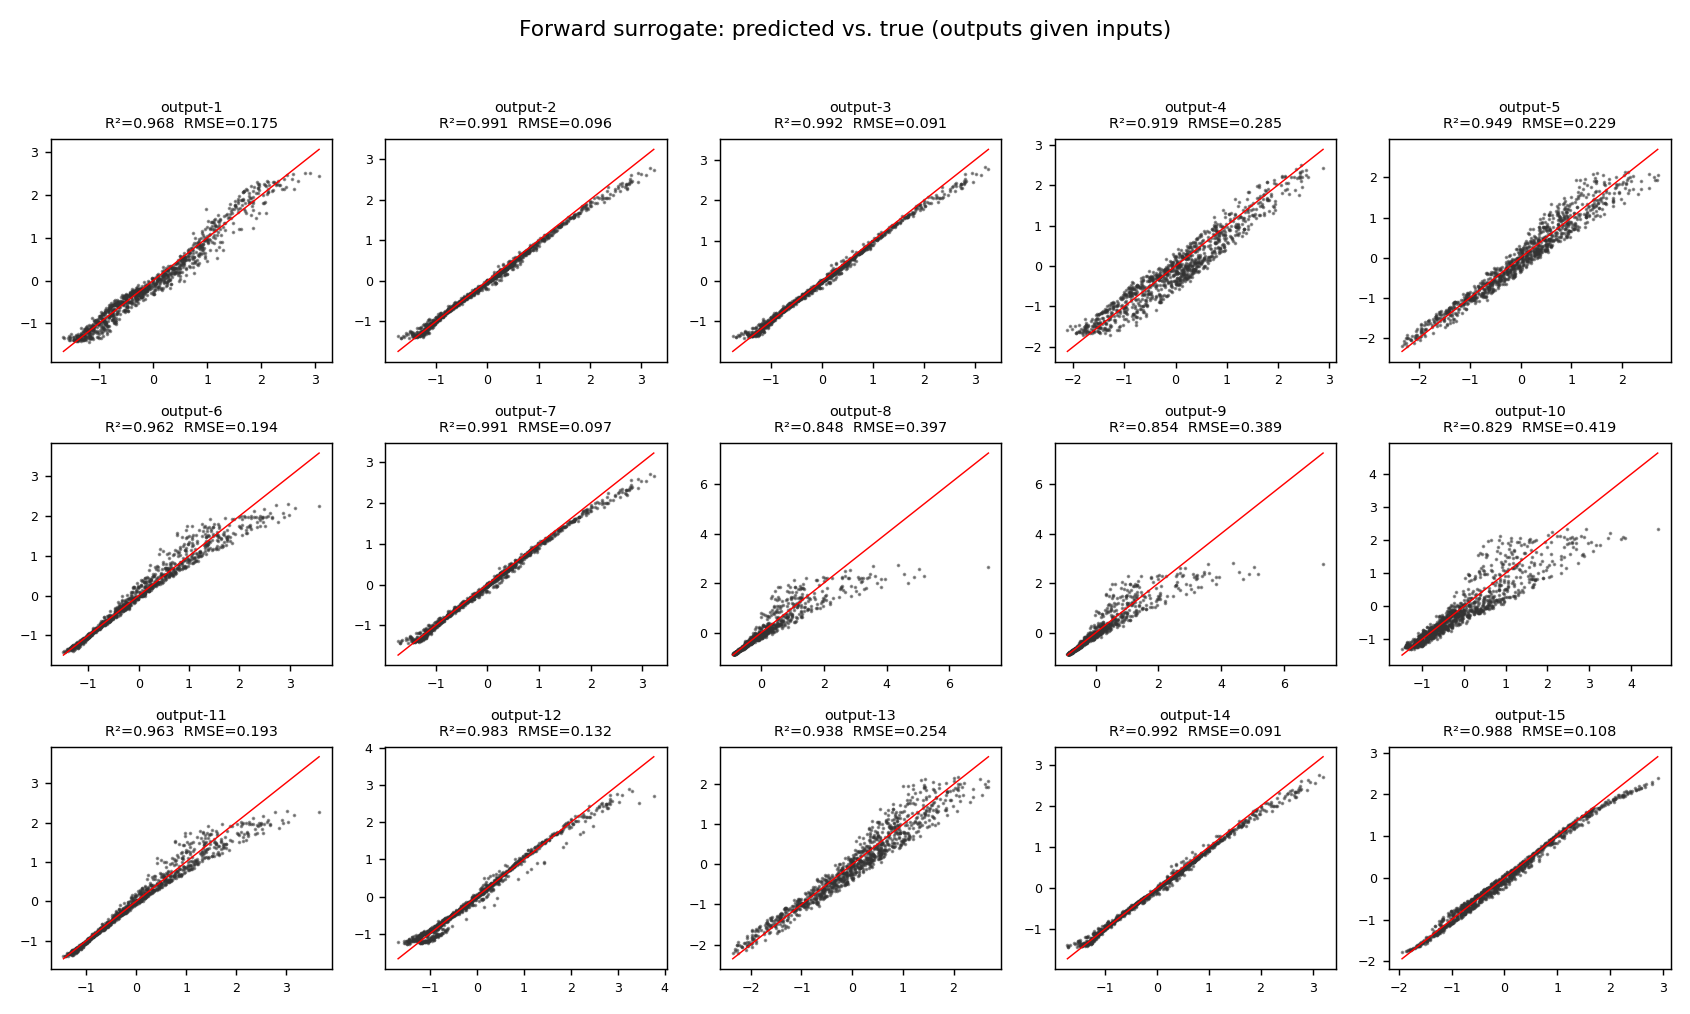
\includegraphics[width=0.97\linewidth]{artifacts/figs/03_forward_scatter.png}
\caption{Forward surrogate: predicted vs.\ true outputs on the 1\,k test
samples. Each panel reports the per-dimension $R^{2}$ and RMSE.}
\label{fig:fwd}
\end{figure}

%==============================================================
\section{Inverse surrogate mode}

Swapping the visibility \textemdash{} 15 outputs visible, 5 inputs masked
\textemdash{} the same network is queried as an inverse surrogate.
Average $R^{2}_{\text{inv}}\!\approx\!0.40$ (Figure~\ref{fig:inv}).
The drop relative to the forward direction is \emph{not} a model failure:
the inverse map is intrinsically one-to-many on this dataset and the
conditional mean is a poor summary of a multi-modal posterior. The honest
output of the network in this regime is the full posterior, shown next.

\begin{figure}[h]\centering
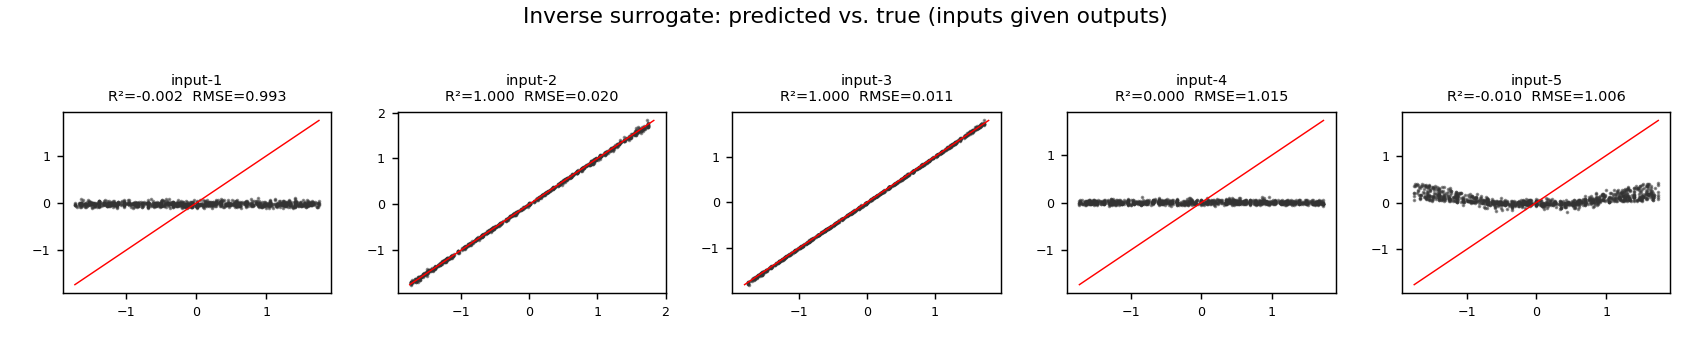
\includegraphics[width=0.97\linewidth]{artifacts/figs/04_inverse_scatter.png}
\caption{Inverse surrogate (point estimates): predicted vs.\ true inputs.
The lower $R^{2}$ values reflect the multi-modal nature of the posterior
$p(\text{input}\mid\text{output})$ rather than a deficiency of the model.}
\label{fig:inv}
\end{figure}

%==============================================================
\section{Bayesian posterior over the inputs}

We pick one held-out sample, treat its 15 output values as
``measurements'', and draw $4\,000$ posterior samples of the 5 inputs by
ancestral sampling in random order (the procedure of Page~11 of the deck).
The resulting corner plot is in Figure~\ref{fig:post}.

\begin{figure}[h]\centering
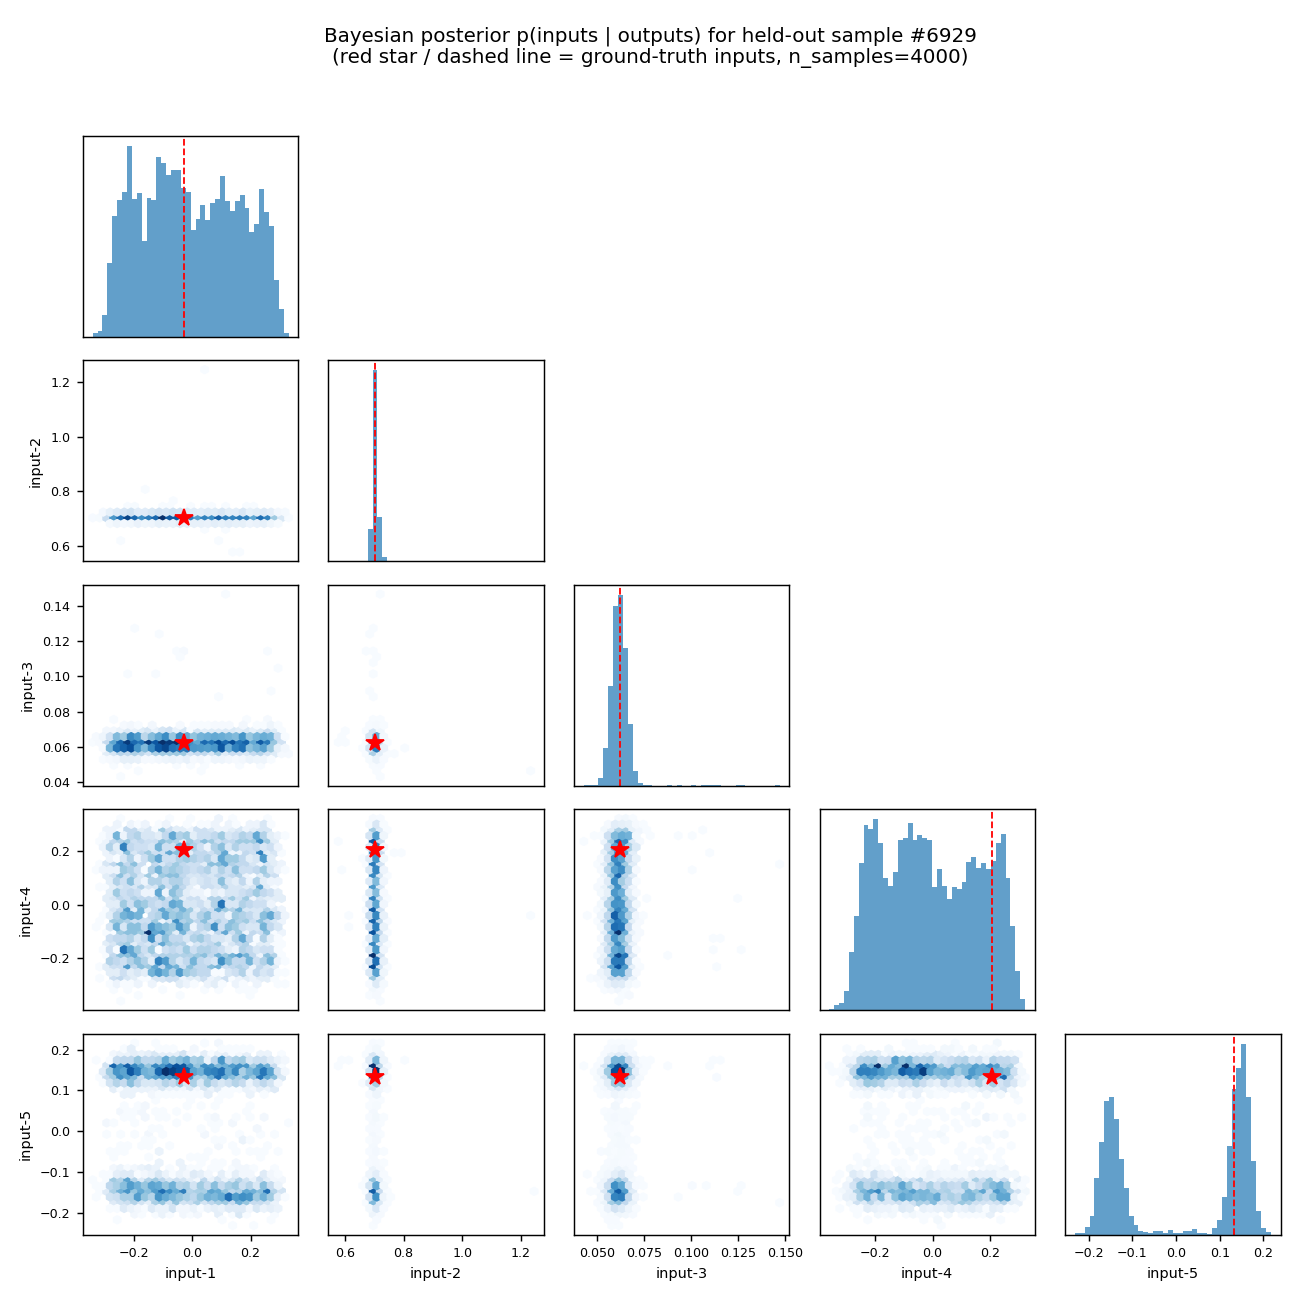
\includegraphics[width=0.85\linewidth]{artifacts/figs/05_posterior_corner.png}
\caption{Bayesian posterior $p(\text{inputs}\mid\text{outputs})$ for one
held-out sample. The ground-truth input vector (red star / dashed line)
falls in a high-density region. The posterior is sharp on
\texttt{input-2} and \texttt{input-3}, broad on \texttt{input-1} /
\texttt{input-4}, and \emph{bimodal} on \texttt{input-5} \textemdash{} a
genuine physical degeneracy that the forward map cannot resolve.}
\label{fig:post}
\end{figure}

%==============================================================
\section{Conditional slice}

Figure~\ref{fig:slice} demonstrates the third use mode of the deck
(``scaling-law / correlation analysis''): we fix \texttt{input-1} to five
different values $c$ and read off the predicted conditional density
$p(\text{output-1}\mid\text{input-1}{=}c)$. The peak position and width
deform smoothly with $c$, exactly the kind of map from which one would
read off a power-law exponent on real ICF data.

\begin{figure}[h]\centering
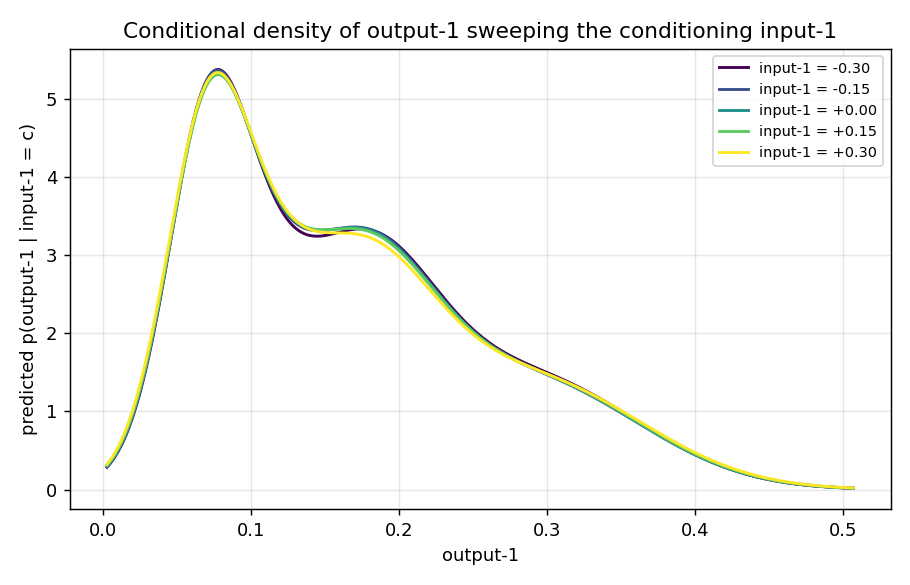
\includegraphics[width=0.78\linewidth]{artifacts/figs/06_conditional_slice.png}
\caption{Sweep of \texttt{input-1} from low (purple) to high (yellow) values
and the resulting predicted conditional density of \texttt{output-1}.}
\label{fig:slice}
\end{figure}

%==============================================================
\section{Summary}

A single, modest 0.20\,M-parameter Transformer trained for 120 epochs on
9\,000 samples reproduces the three capabilities advertised in the slide
deck:
\begin{enumerate}
  \item it fits the marginal data densities accurately for all 20
        quantities (Figure~\ref{fig:marg});
  \item it acts as a high-quality forward surrogate
        ($R^{2}{\approx}0.94$, Figure~\ref{fig:fwd});
  \item via ancestral sampling it produces a calibrated Bayesian posterior
        for any subset of variables given any other subset
        (Figures~\ref{fig:post}, \ref{fig:slice}).
\end{enumerate}
The same checkpoint can therefore answer ``forward'', ``inverse'',
``constrained-design'' and ``scaling-law'' queries on
\texttt{combined\_data.xlsx} without any retraining.

\bigskip
\noindent\small
Reproduction: \texttt{python train.py \&\& python evaluate.py \&\& tectonic report.tex}

\end{document}
